\documentclass{article}

\usepackage{graphicx}
\usepackage{tikz}
\usepackage{tikzsymbols}
\usetikzlibrary{calc,patterns,shapes.geometric}
\pagestyle{empty}
\usepackage[margin=0pt]{geometry}
\geometry{papersize={14in,12in}}

\def\centerarc[#1](#2)(#3:#4:#5){\draw[#1] ($(#2)+({#5*cos(#3)},{#5*sin(#3)})$) arc (#3:#4:#5);}

\begin{document}
	\begin{figure}
		\centering
		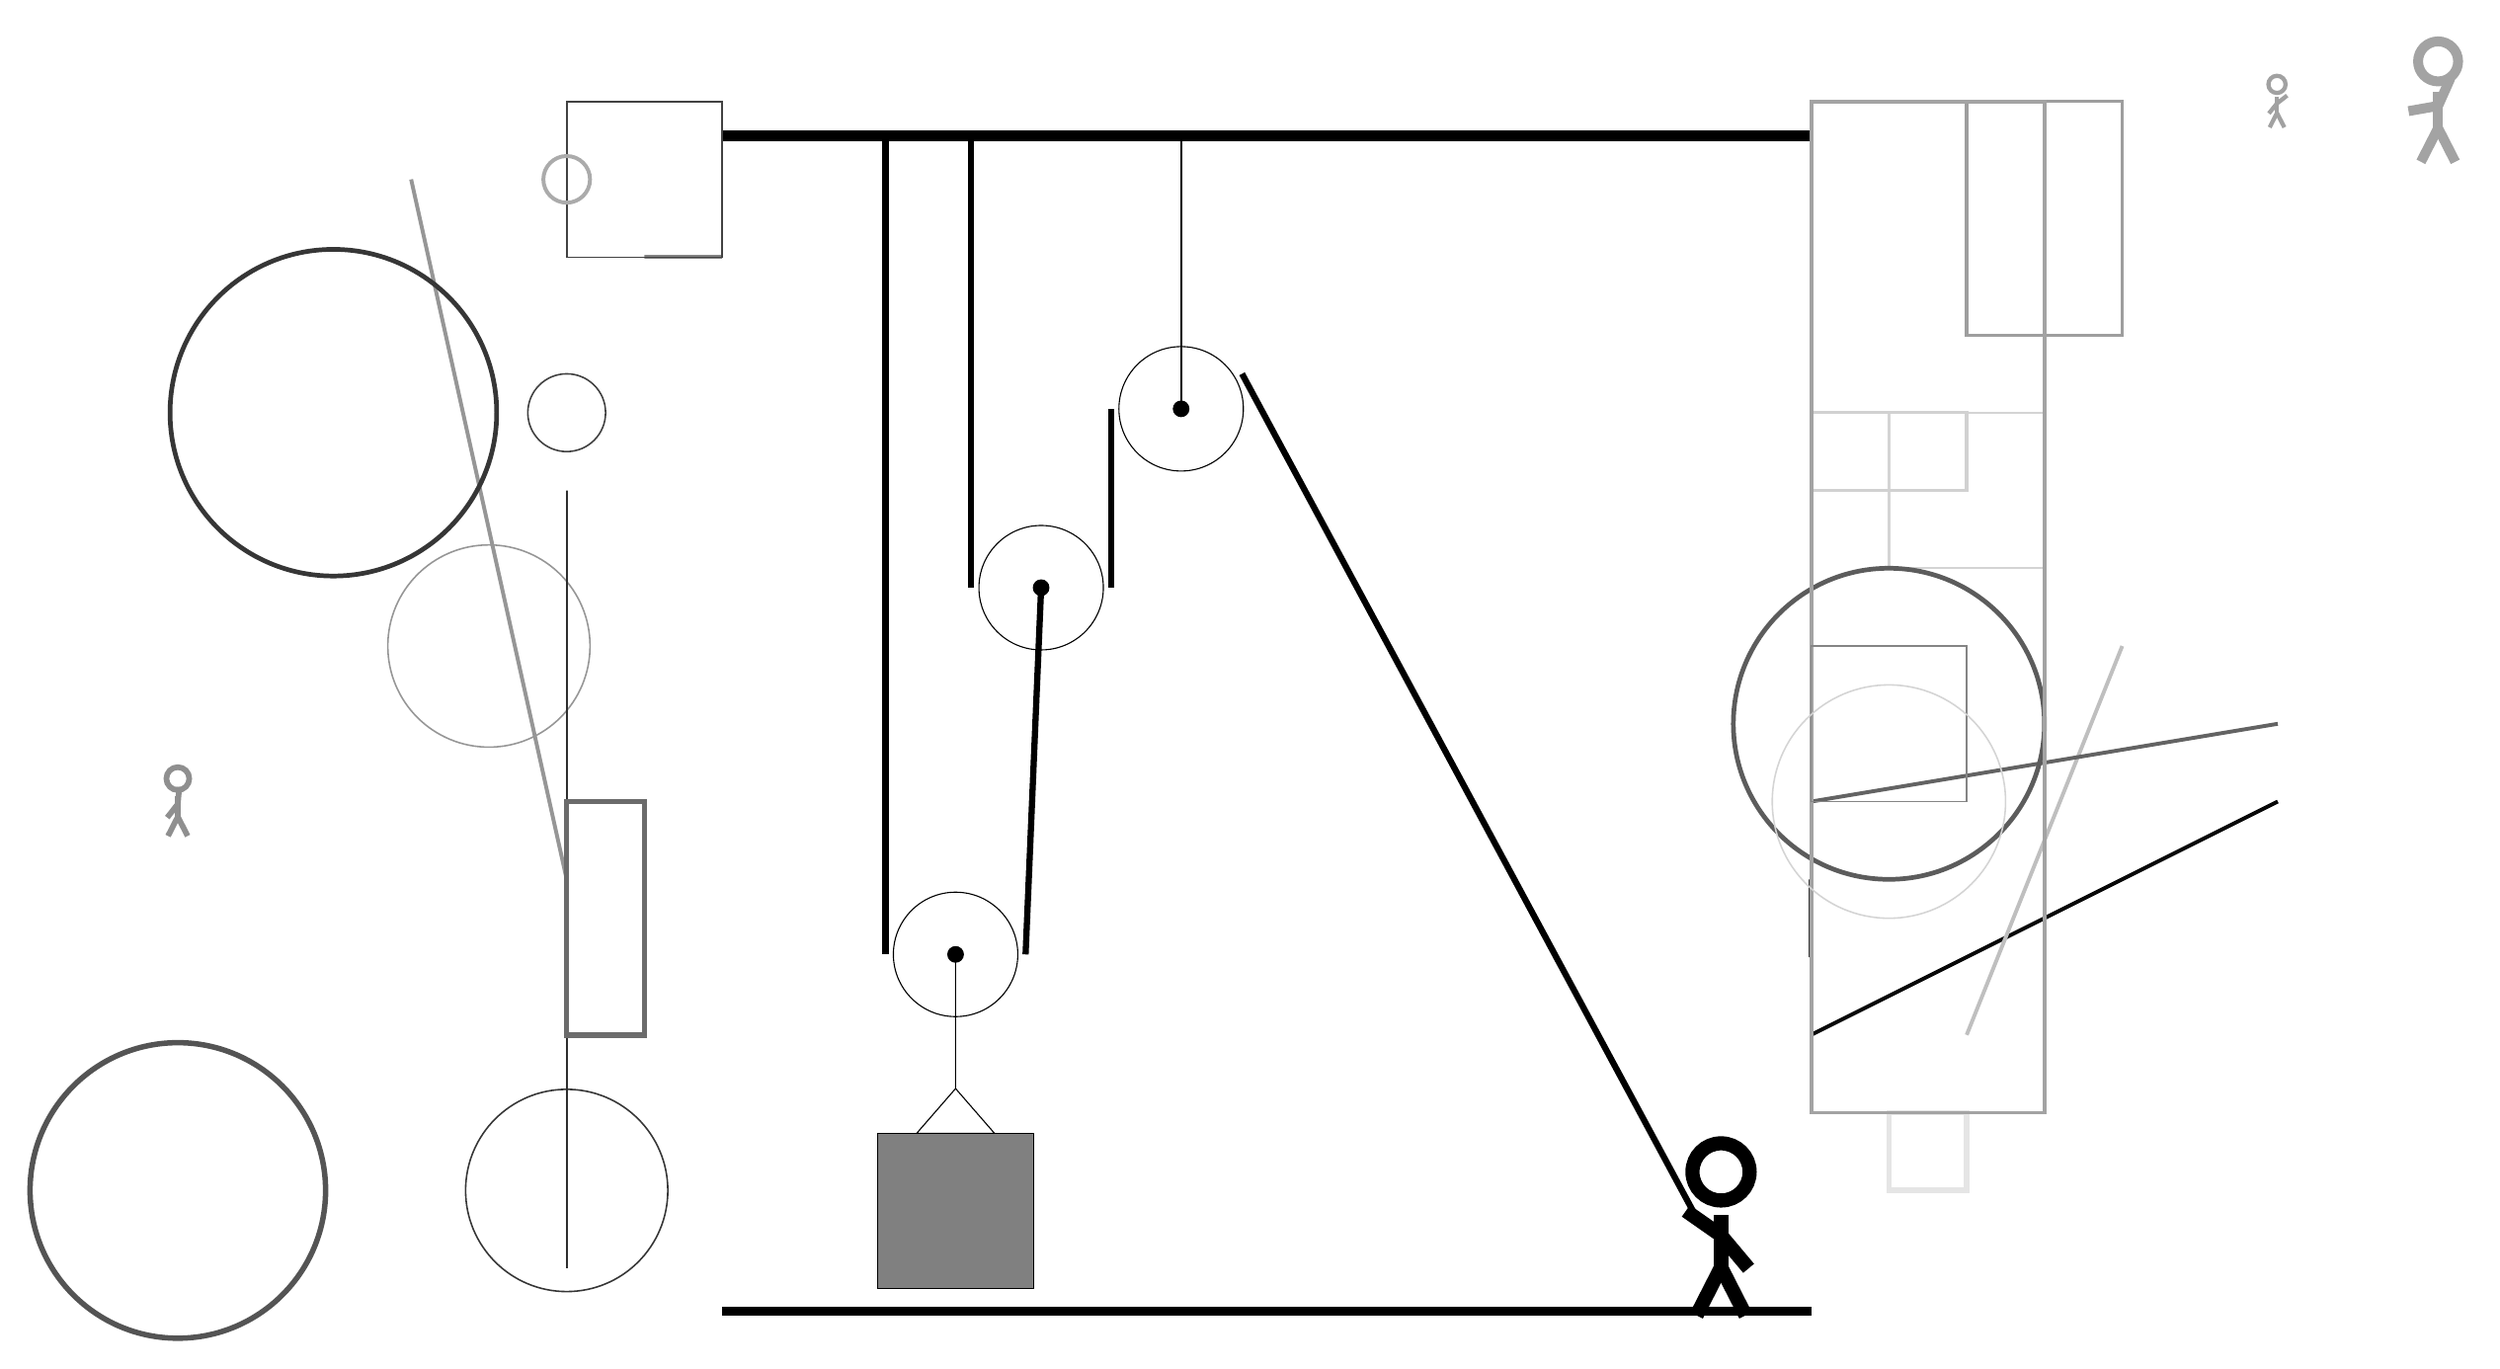
\begin{tikzpicture}
			%%%%% START %%%%%
			
			\draw[fill=black] (-2, 11.5) rectangle (12, 11.625);
			
			\draw (1, 1.035) circle (0.8);
			\draw[fill=black] (1, 1.035) circle (0.1);
			
			\draw (2.1, 5.75) circle (0.8);
			\draw[fill=black] (2.1, 5.75) circle (0.1);
			
			\draw (3.9, 8.05) circle (0.8);
			\draw[fill=black] (3.9, 8.05) circle (0.1);
			\draw[thick] (3.9, 8.05) -- (3.9, 11.5);
			
			\draw (1, 1.035) -- (1, -0.69) -- (0.5, -1.265) -- (1.5, -1.265) -- (1, -0.69);
			\draw[fill=black!50] (0, -1.265) rectangle (2, -3.265);
			
			\draw[line width=0.8mm] (0.1, 11.5) -- (0.1, 1.035);
			\centerarc[line width=0.8mm](1, 1.035)(180:360:0.9);
			\draw[line width=0.8mm](1.9, 1.035) -- (2.1, 5.75);
			\draw[line width=0.8mm] (1.2, 11.5) -- (1.2, 5.75);
			\centerarc[line width=0.8mm](2.1, 5.75)(180:360:0.9);
			\draw[line width=0.8mm](3.0, 5.75) -- (3.0, 8.05);
			\centerarc[line width=0.8mm](3.9, 8.05)(30:180:0.9);
			\draw[line width=0.8mm] (4.683, 8.5) -- (10.5, -2.3);
			
			\node at (10.8, -2.5) {\Strichmaxerl[10][-35][-50]};
			
			\draw[line width=0.5mm, color=black!97](12, 0) -- (18, 3);
			
			\draw [line width=0.2mm, color=black!41](-5, 5) circle (1.3);
			\node[line width=0.7mm, color=black!37] at (18, 12) {\Strichmaxerl[3][51][38]};
			\draw[line width=0.7mm, color=black!80] (12, 2) rectangle (12, 1);
			
			\draw[line width=0.3mm, color=black!17] (13, 8) rectangle (15, 6);
			\node[line width=0.2mm, color=black!44] at (-9, 3) {\Strichmaxerl[4][52][85]};
			
			\draw[line width=0.5mm, color=black!25](16, 5) -- (14, 0);
			\draw[line width=0.4mm, color=black!38] (14, 9) rectangle (16, 12);
			\draw[line width=0.5mm, color=black!41](-6, 11) -- (-4, 2);
			\draw [line width=0.2mm, color=black!79](-4, -2) circle (1.3);
			\draw[line width=0.2mm, color=black!82] (-4, 7) rectangle (-4, -3);
			
			\draw[line width=0.5mm, color=black!61](12, 3) -- (18, 4);
			\draw[line width=0.7mm, color=black!58] (-4, 0) rectangle (-3, 3);
			\draw [line width=0.6mm, color=black!64](13, 4) circle (2.0);
			\draw[line width=0.5mm, color=black!49] (-3, 10) rectangle (-2, 10);
			\draw [line width=0.7mm, color=black!67](-9, -2) circle (1.9);
			\draw [line width=0.4mm, color=black!60](13, 7) circle (0.0);
			\draw[line width=0.7mm, color=black!10] (14, -2) rectangle (13, -1);
			\draw[line width=0.4mm, color=black!18] (14, 7) rectangle (12, 8);
			\draw[line width=0.5mm, color=black!36] (12, 12) rectangle (15, -1);
			\draw[line width=0.2mm, color=black!74] (-2, 12) rectangle (-4, 10);
			
			\node[line width=0.7mm, color=black!36] at (20, 12) {\Strichmaxerl[7][10][66]};
			
			\draw [line width=0.6mm, color=black!79](-7, 8) circle (2.1);
			\draw [line width=0.2mm, color=black!75](-4, 8) circle (0.5);
			\draw[line width=0.2mm, color=black!48] (12, 5) rectangle (14, 3);
			\draw [line width=0.5mm, color=black!33](-4, 11) circle (0.3);
			
			\draw [line width=0.2mm, color=black!17](13, 3) circle (1.5);
			
			\draw[fill=black] (-2, -3.5) rectangle (12, -3.6);
			
			%%%%% END %%%%%
		\end{tikzpicture}
	\end{figure}	
\end{document}